%%%%%%%%%%%%%%%%%%%%%%%%%%%%%%%%%%%%%%%%%
% KOMA-Script Presentation
% LaTeX Template
% Version 1.1 (18/10/15)
%
% This template has been downloaded from:
% http://www.LaTeXTemplates.com
%
% Original Authors:
% Marius Hofert (marius.hofert@math.ethz.ch)
% Markus Kohm (komascript@gmx.info)
% Described in the PracTeX Journal, 2010, No. 2
%
% License:
% CC BY-NC-SA 3.0 (http://creativecommons.org/licenses/by-nc-sa/3.0/)
%
%%%%%%%%%%%%%%%%%%%%%%%%%%%%%%%%%%%%%%%%%

%----------------------------------------------------------------------------------------
%	PACKAGES AND OTHER DOCUMENT CONFIGURATIONS
%----------------------------------------------------------------------------------------

\documentclass[
%paper=128mm:96mm, % The same paper size as used in the beamer class
paper=192mm:144mm, % The same paper size as used in the beamer class
fontsize=12pt, % Font size
pagesize, % Write page size to dvi or pdf
parskip=half-, % Paragraphs separated by half a line
]{scrartcl} % KOMA script (article)

\linespread{1.12} % Increase line spacing for readability
%------------------------------------------------
% Colors
\usepackage{xcolor}	 % Required for custom colors
% Define a few colors for making text stand out within the presentation
\definecolor{mygreen}{RGB}{44,85,17}
\definecolor{myblue}{RGB}{34,31,217}
\definecolor{mybrown}{RGB}{194,164,113}
\definecolor{myred}{RGB}{255,66,56}
% Use these colors within the presentation by enclosing text in the commands below
\newcommand*{\mygreen}[1]{\textcolor{mygreen}{#1}}
\newcommand*{\myblue}[1]{\textcolor{myblue}{#1}}
\newcommand*{\mybrown}[1]{\textcolor{mybrown}{#1}}
\newcommand*{\myred}[1]{\textcolor{myred}{#1}}
%------------------------------------------------

%------------------------------------------------
% Margins
\usepackage[ % Page margins settings
includeheadfoot,
top=3.5mm,
bottom=3.5mm,
left=15.5mm,
right=15.5mm,
headsep=6.5mm,
footskip=8.5mm
]{geometry}
%------------------------------------------------

%------------------------------------------------
% Fonts
\usepackage[T1]{fontenc}	 % For correct hyphenation and T1 encoding
\usepackage{lmodern} % Default font: latin modern font
%\usepackage{fourier} % Alternative font: utopia
%\usepackage{charter} % Alternative font: low-resolution roman font
\renewcommand{\familydefault}{\sfdefault} % Sans serif - this may need to be commented to see the alternative fonts
%------------------------------------------------

%------------------------------------------------
% Various required packages
\usepackage{amsthm} % Required for theorem environments
\usepackage{bm} % Required for bold math symbols (used in the footer of the slides)
\usepackage{graphicx} % Required for including images in figures
\usepackage{tikz} % Required for colored boxes
\usepackage{booktabs} % Required for horizontal rules in tables
\usepackage{multicol} % Required for creating multiple columns in slides
\usepackage{lastpage} % For printing the total number of pages at the bottom of each slide
\usepackage[ngerman]{babel} % Document language - required for customizing section titles
\usepackage{microtype} % Better typography
\usepackage{tocstyle} % Required for customizing the table of contents
\usepackage[utf8]{inputenc} %Umlaute
\usepackage{wrapfig}
\usepackage{framed}
\usepackage{amsmath} %für \text{} align
\usepackage{amsfonts} %für mathbb
\usepackage[hidelinks]{hyperref}
\usepackage{lipsum}
%------------------------------------------------

%------------------------------------------------
% Slide layout configuration
\usepackage{scrpage2} % Required for customization of the header and footer
\pagestyle{scrheadings} % Activates the pagestyle from scrpage2 for custom headers and footers
\clearscrheadfoot % Remove the default header and footer
\setkomafont{pageheadfoot}{\normalfont\color{black}\sffamily} % Font settings for the header and footer

% Sets vertical centering of slide contents with increased space between paragraphs/lists
\makeatletter
\renewcommand*{\@textbottom}{\vskip \z@ \@plus 1fil}
\newcommand*{\@texttop}{\vskip \z@ \@plus .25fil}
\addtolength{\parskip}{\z@\@plus .25fil}
\makeatother

% Remove page numbers and the dots leading to them from the outline slide
\makeatletter
\newtocstyle[noonewithdot]{nodotnopagenumber}{\settocfeature{pagenumberbox}{\@gobble}}
\makeatother
\usetocstyle{nodotnopagenumber}

\AtBeginDocument{\renewcaptionname{ngerman}{\contentsname}{\Large Überblick}} % Change the name of the table of contents
%------------------------------------------------

%------------------------------------------------
% Header configuration - if you don't want a header remove this block
\ihead{
\hspace{-2mm}
\begin{tikzpicture}[remember picture,overlay]
\node [xshift=\paperwidth/2,yshift=-\headheight] (mybar) at (current page.north west)[rectangle,fill,inner sep=0pt,minimum width=\paperwidth+60,minimum height=2\headheight,top color=mygreen!64,bottom color=mygreen]{}; % Colored bar
\node[below of=mybar,yshift=3.3mm,rectangle,shade,inner sep=0pt,minimum width=256mm,minimum height =1.5mm,top color=black!50,bottom color=white]{}; % Shadow under the colored bar
shadow
\end{tikzpicture}
\color{white}\textbf{\runninghead}} % Header text defined by the \runninghead command below and colored white for contrast
%------------------------------------------------

%------------------------------------------------
% Footer configuration
\setlength{\footheight}{8mm} % Height of the footer
\addtokomafont{pagefoot}{\footnotesize} % Small font size for the footnote

\ifoot{% Left side
\hspace{-2mm}
\begin{tikzpicture}[remember picture,overlay]
\node [xshift=\paperwidth/2,yshift=\footheight] at (current page.south west)[rectangle,fill,inner sep=0pt,minimum width=\paperwidth+60,minimum height=3pt,top color=mygreen,bottom color=mygreen]{}; % Green bar
\end{tikzpicture}
\myauthor\ \ \raisebox{0.2mm}{$\bm{\vert}$}\ \ \myuni%\ \ \raisebox{0.2mm}{$\bm{\vert}$}\ \ \myemail % Left side text
}

\ofoot[\pagemark/\pageref{LastPage}\hspace{-2mm}]{\pagemark/\pageref{LastPage}\hspace{-2mm}} % Right side
%------------------------------------------------

%------------------------------------------------
% Section spacing - deeper section titles are given less space due to lesser importance
\usepackage{titlesec} % Required for customizing section spacing
\titlespacing{\section}{0mm}{0mm}{0mm} % Lengths are: left, before, after
\titlespacing{\subsection}{0mm}{0mm}{-1mm} % Lengths are: left, before, after
\titlespacing{\subsubsection}{0mm}{0mm}{-2mm} % Lengths are: left, before, after
\setcounter{secnumdepth}{0} % How deep sections are numbered, set to no numbering by default - change to 1 for numbering sections, 2 for numbering sections and subsections, etc
%------------------------------------------------

%------------------------------------------------
% Theorem style
\newtheoremstyle{mythmstyle} % Defines a new theorem style used in this template
{0.5em} % Space above
{0.5em} % Space below
{} % Body font
{} % Indent amount
{\sffamily\bfseries} % Head font
{} % Punctuation after head
{\newline} % Space after head
{\thmname{#1}\ \thmnote{(#3)}} % Head spec
	
\theoremstyle{mythmstyle} % Change the default style of the theorem to the one defined above
\newtheorem{theorem}{Theorem}[section] % Label for theorems
\newtheorem{remark}[theorem]{Remark} % Label for remarks
\newtheorem{algorithm}[theorem]{Algorithm} % Label for algorithms
\makeatletter % Correct qed adjustment
%------------------------------------------------

%------------------------------------------------
% The code for the box which can be used to highlight an element of a slide (such as a theorem)
\newcommand*{\mybox}[2]{ % The box takes two arguments: width and content
\par\noindent
\begin{tikzpicture}[mynodestyle/.style={rectangle,draw=mygreen,thick,inner sep=2mm,text justified,top color=white,bottom color=white,above}]\node[mynodestyle,at={(0.5*#1+2mm+0.4pt,0)}]{ % Box formatting
\begin{minipage}[t]{#1}
#2
\end{minipage}
};
\end{tikzpicture}
\par\vspace{-1.3em}}
%------------------------------------------------

%----------------------------------------------------------------------------------------
%	PRESENTATION INFORMATION
%----------------------------------------------------------------------------------------
\usepackage{nameref}
\newcommand*{\mytitle}{Simulation of Inextensible Hair and Fur} % Title
\newcommand*{\runninghead}{\@currentlabelname} % Running head displayed on almost all slides
\newcommand*{\myauthor}{Tom Möbert \& Mathias Putz} % Presenters name(s)
\newcommand*{\mydate}{2. February 2017} % Presentation date
\newcommand*{\myuni}{Simulation of Inextensible Hair and Fur} % University or department
\newcommand*{\myemail}{} % University or department
\newcommand\invisiblesection[1]{%
  \refstepcounter{section}%
  \addcontentsline{toc}{section}{#1}%
  \sectionmark{#1}
  \def\@currentlabelname{#1}
  }
 


%----------------------------------------------------------------------------------------

\begin{document}

%----------------------------------------------------------------------------------------
%	TITLE SLIDE
%----------------------------------------------------------------------------------------

% Title slide - you may have to tweak a few of the numbers if you wish to make changes to the layout
\thispagestyle{empty} % No slide header and footer
\begin{tikzpicture}[remember picture,overlay] % Background box
\node [xshift=\paperwidth/2,yshift=\paperheight/2+95] at (current page.south west)[rectangle,fill,inner sep=0pt,minimum width=\paperwidth+60,minimum height=\paperheight/3,top color=mygreen,bottom color=mygreen]{}; % Change the height of the box, its colors and position on the page here
\end{tikzpicture}
% Text within the box
\begin{flushright}
%\vspace{2.6cm}
\vspace{-10mm}
\color{white}\sffamily
{\bfseries\Large\mytitle\par} % Title
\vspace{0.5cm}
\normalsize
\myauthor\par % Author name
\mydate\par % Date
\vfill
\end{flushright}
\begin{figure}[h]
\begin{center}

\includegraphics[width=4cm,height=4.5cm]{Bilder/Uni-Jena-logo.png}
\end{center}	
\end{figure}

\newpage
%\clearpage

%%----------------------------------------------------------------------------------------
%%	TABLE OF CONTENTS
%%----------------------------------------------------------------------------------------
%
%%\thispagestyle{empty} % No slide header and footer
%
%\small\tableofcontents % Change the font size and print the table of contents - it may be useful to shrink the font size further if the presentation is full of sections
%% To exclude sections/subsections from the table of contents, put an asterisk after \(sub)section like so: \section*{Section Name}
%
%\clearpage

%----------------------------------------------------------------------------------------
%	PRESENTATION SLIDES
%----------------------------------------------------------------------------------------

\section{\color{white}What we do}
\begin{itemize}
%\setlength\itemsep{-3mm}
\item We focus on the fast simulation of hair and fur on animated characters.
\item \textbf{Where is it used?} Films, computer games or related
\item \textbf{Whats the difficulty?} The sheer number of hair strands and the fact that each hair is inextensible. Keeping thousands of deformable objects from being stretched is computationally expensive.
\item To do this in \textbf{real time} and \textbf{naturally}.
\end{itemize}

\begin{center}
\href{https://youtu.be/zB8Fqbfrrpo?t=106}{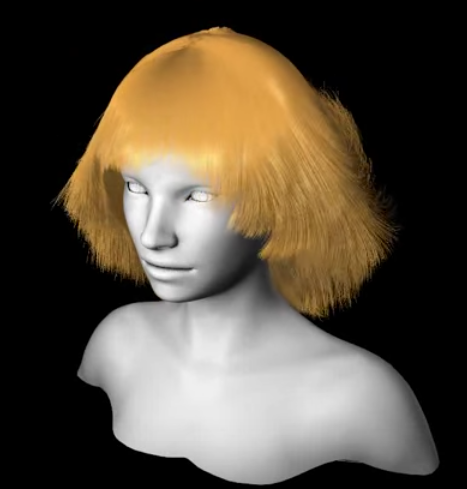
\includegraphics[scale=0.4]{Bilder/1.png}}
\end{center}


\clearpage

%----------------------------------------------------------------------------------------
%	3
%----------------------------------------------------------------------------------------

\section{\color{white}Model}

The following algorithm is described in:\\ \href{http://matthias-mueller-fischer.ch/publications/FTLHairFur.pdf}{M. Müller, T.Y. Kim, N. Chentanez,  Fast Simulation of Inextensible Hair and Fur, Darmstadt, Germany, December 6-7 2012}.

\begin{itemize}
\setlength\itemsep{-5mm}
\item We model a single hair by a chain of particles that is attached
at one end ($x_1,...,x_n$).
\item All particles have the same distance $l_0$ in between.
\item We start at a particle that violate the distance constraints, commonly $x_1$.
\item We iterate through all the particles once and move the particles such that all the constraints are satisfied.
\end{itemize}


\clearpage

%----------------------------------------------------------------------------------------
%	4
%----------------------------------------------------------------------------------------

\section{\color{white}How to fulfill the constraints}

Process called Follow-The-Leader (a).
\begin{itemize}
\setlength\itemsep{-5mm}
\item Process the particles in the order from 2 to n.
\item Particle $i$ has to be on a sphere with radius $l_0$ around particle $i-1$.
\item Choose the point on the sphere that is closest to the original position $x_i$.
\end{itemize}

\begin{center}
\begin{framed}
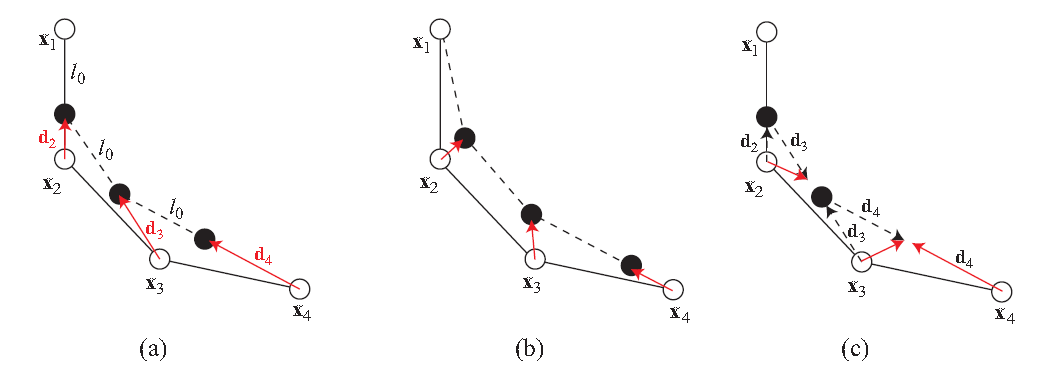
\includegraphics[scale=0.5]{Bilder/2.png}
\end{framed}
\end{center}


\clearpage

%----------------------------------------------------------------------------------------
%	5
%----------------------------------------------------------------------------------------

\section{\color{white}To be dynamic}

\vspace{-1cm}
\begin{itemize}
\setlength\itemsep{-4mm}
\item Need to store and update velocities $v_1,...,v_n$ along with the positions.
\item A way to derive the velocity updates from the position updates is called\\ \textbf{Position Based Dynamics (PBD)} (b).
\end{itemize}

\vspace{-1cm}
\begin{eqnarray}
x + \Delta tv + \Delta t^2f \rightarrow p\\
solve\_constraints(p) \rightarrow p\\
\frac{x - p}{\Delta t} \rightarrow v\\
p \rightarrow x
\end{eqnarray}

\begin{center}
\begin{framed}
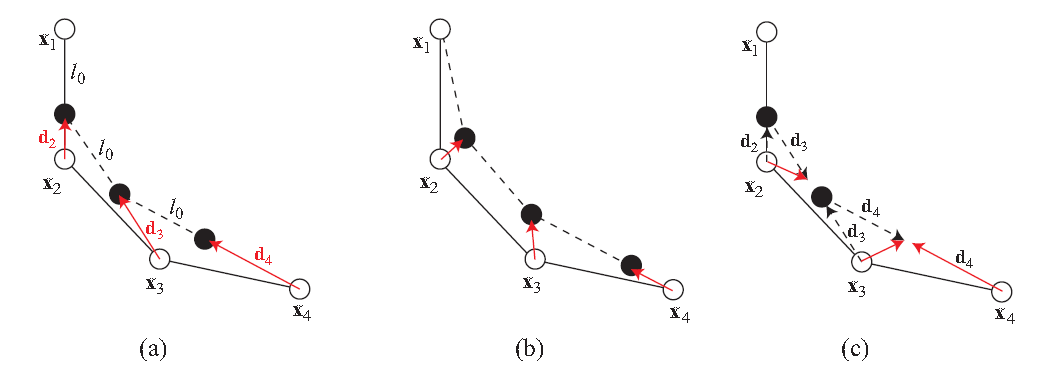
\includegraphics[scale=0.5]{Bilder/2.png}
\end{framed}
\end{center}


\clearpage

%----------------------------------------------------------------------------------------
%	6
%----------------------------------------------------------------------------------------

\section{\color{white}What happened}

\begin{wrapfigure}{r}{0.55\textwidth}
	\vspace{-1cm}
    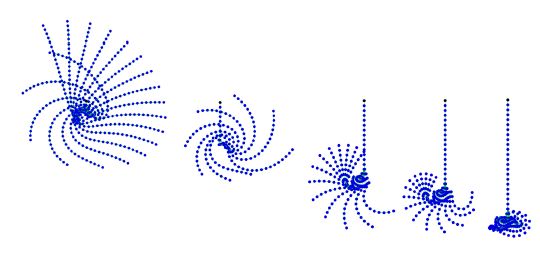
\includegraphics[scale=0.6]{Bilder/3.png}
\end{wrapfigure}

Without respect to the mass of the particles, the method above ends up in a strange behavior.\\
To fix that bug we need a \textbf{velocity correction} by using damping (c).

\vspace{-1cm}
\begin{eqnarray}
\frac{x_i - p_i}{\Delta t} + s_{damping}\frac{-d_{i+1}}{\Delta t} \rightarrow v_i
\end{eqnarray}

With the correction vector $d_i$ and $s_{damping} \in [0,1]$.

\begin{center}
\begin{framed}
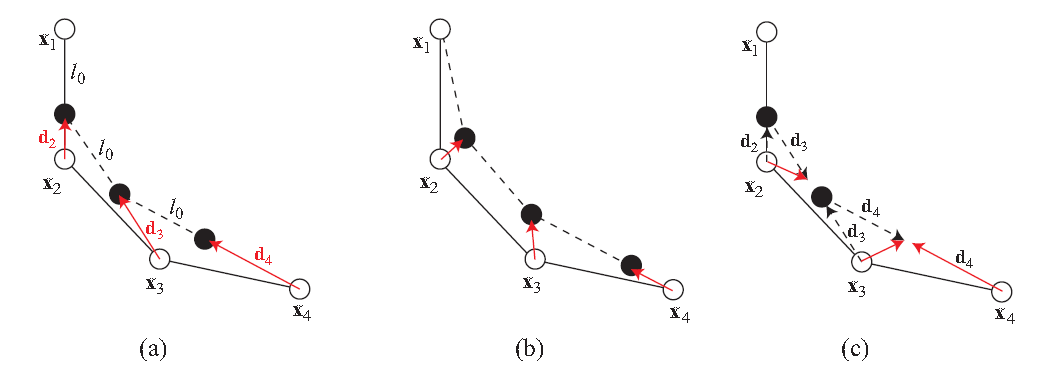
\includegraphics[scale=0.45]{Bilder/2.png}
\end{framed}
\end{center}

\clearpage

%----------------------------------------------------------------------------------------
%	7
%----------------------------------------------------------------------------------------

\section{\color{white}Our implementation}

\begin{itemize}
\setlength\itemsep{-5mm}
\item openGL and openMP is used
\item implementation of 2 different algorithms
\item display and save simulation
\item used aligned data-structure (64 byte without padding) for all vertexes
\item debug vs release build speedup: 6 @ PBD, 16 @ FTL
\item measured average time of 10000 pictures with 1000 strands and 50 vertexes each
\item speedup:
\end{itemize}

\begin{center}
\begin{tabular}{|c|c|c|c|c|c|}
\hline
threads & 2 & 4 & 8 & 12 & 16 \\
\hline
FTL & 1.4 & 2.6 & 5.1 & 7.6 & 9.7\\
\hline
PBD & 1.4 & 2.6 & 5.2 & 7.6 & 10.0\\
\hline
\end{tabular}
\end{center}

\clearpage

%----------------------------------------------------------------------------------------
%	8
%----------------------------------------------------------------------------------------

\section{\color{white}Times}

\begin{center}
\begin{framed}
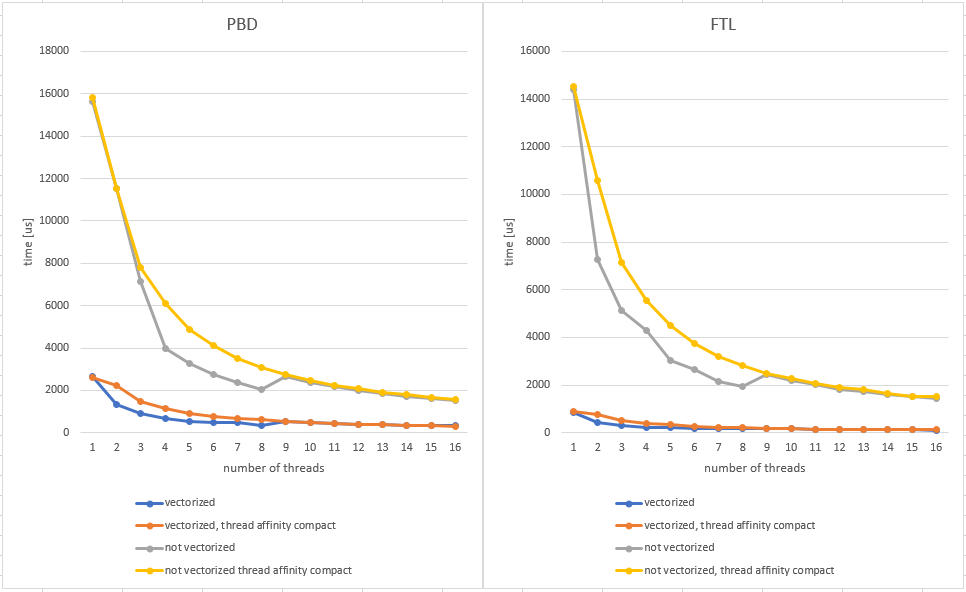
\includegraphics[scale=0.6]{Bilder/4.png}
\end{framed}
\end{center}


\clearpage

%----------------------------------------------------------------------------------------
%	9
%----------------------------------------------------------------------------------------

\begin{center}
%\begin{framed}
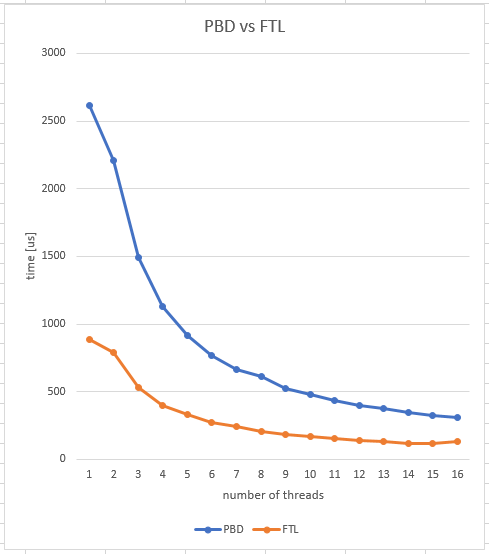
\includegraphics[scale=0.65]{Bilder/5.png}
%\end{framed}
\end{center}


\clearpage

%----------------------------------------------------------------------------------------
%	??
%----------------------------------------------------------------------------------------

\thispagestyle{empty} % No slide header and footer

\begin{tikzpicture}[remember picture,overlay] % Background box
\node [xshift=\paperwidth/2,yshift=\paperheight/2] at (current page.south west)[rectangle,fill,inner sep=0pt,minimum width=\paperwidth,minimum height=\paperheight/3,top color=mygreen,bottom color=mygreen]{}; % Change the height of the box, its colors and position on the page here
\end{tikzpicture}
% Text within the box
\begin{flushright}
\vspace{2.6cm}
\color{white}\sffamily
%{\bfseries\LARGE Questions?\par} % Request for questions text
\vfill
\end{flushright}

%----------------------------------------------------------------------------------------

\end{document}